\clearpage

\section{Local Oscillator}

\begin{tcolorbox}	
	\begin{tabular}{p{2.75cm} p{0.2cm} p{10.5cm}} 	
		\textbf{Header File}   &:& local\_oscillator.h \\
		\textbf{Source File}   &:& local\_oscillator.cpp \\
        \textbf{Version}       &:& 20180815 (Pedro Loureiro)\\
	\end{tabular}
\end{tcolorbox}

This block simulates a local oscillator, which consists on an electronic oscillator used to generate a signal with a constant power, initial phase and Wavelength,  however we can simulate a non-ideal local oscillator by putting a non-zero value for laserLineWidth, frequencyMismatch or laserRIN. It will produce one output complex signal and it doesn't have input signals. By the figure \ref{Blocos} its possible to see the two local oscillators in the Block diagram.

\begin{figure}[H]
	\centering
	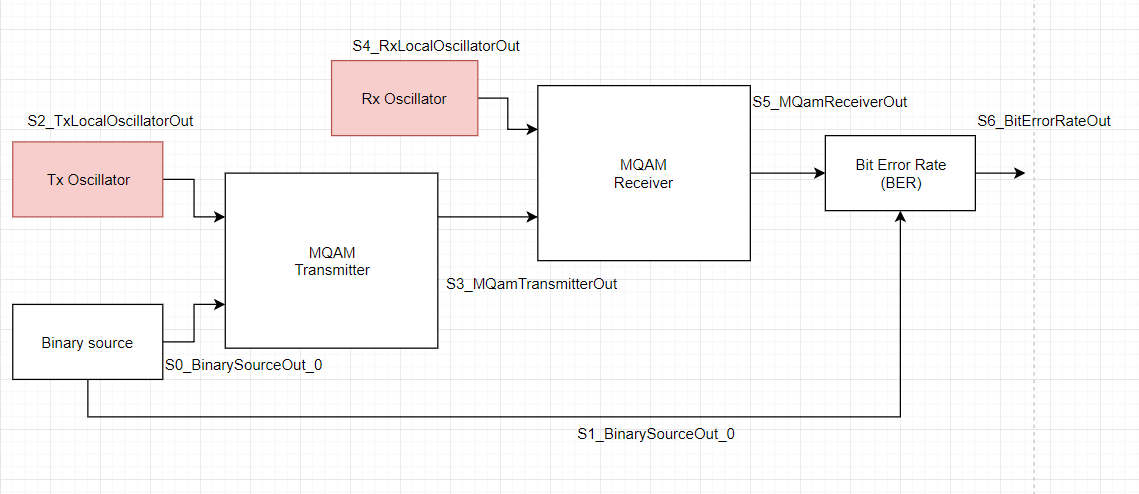
\includegraphics[scale=0.75]{./lib/local_oscillator/Figures/Diagrama_Blocos.png}
	\caption{Block diagram of a transmission system}\label{Blocos}
\end{figure}

\subsection*{Functional description}

This block hasn't inputs and has one output. It generates a complex signal, as can be seen in the following equation:
\begin{equation*}
Out=\sqrt{\frac{Power+Intnoise}{2}}e^{i*phase}
\end{equation*}
The phase depends on the initial phase (input parameter), on the phase Noise (depends on the laserLineWidth) and on the frequencyMismatch. On the other hand Intnoise depends on laserRIN. In the case of no noise the output signal will only be: \newline
\begin{equation*}
Out=\sqrt{\frac{Power}{2}}e^{i*Inphase}
\end{equation*}

\subsection*{Input Signals}

\subparagraph*{Number:} 0

\subsection*{Output Signals}

\subparagraph*{Number:} 1

\subparagraph*{Type:} The Laser emits an optical signal.\par
Transmitter local Oscillator - S2\_TxLocalOscillatorOut\par
Receiver local Oscillator - S4\_RxLocalOscillatorOut

\subsection*{Input Parameters}
This block has set of functions that allow the user to change the basic configuration of the Local Oscillator. The input parameters are summarized in table \ref{table:LO_in_par}.
\begin{table}[H]
	\centering
	\begin{tabular}{|c|c|c|c|cccc}
		\cline{1-4}
		\textbf{Parameter} & \textbf{Type} & \textbf{Values} &   \textbf{Default}& \\ \cline{1-4}
		opticalPower & double & any & $1\text{*10}-3$ \\ \cline{1-4}
		outputOpticalWavelength & double & any & $1550\text{*10}-9$ \\ \cline{1-4}
		outputOpticalFrequency & double & any &  $\frac{SPEED\_OF\_LIGHT}{outputOpticalWavelength} $ \\ \cline{1-4}
		phase & double & $\in \left[0,\frac{\pi}{2}\right]$ & $0$ \\ \cline{1-4}
		samplingPeriod & double & any & $0.0$ \\ \cline{1-4}
        symbolPeriod   & double & any & $0.0$ \\ \cline{1-4}
        signaltoNoiseRatio & double & any & $0.0$ \\ \cline{1-4}
        laserLineWidth$^1$ & double & any & $0.0$ \\ \cline{1-4}
        laserRIN$^2$      & double & any & $0.0$ \\ \cline{1-4}
        frequencyMismatch & double & any & $0.0$ \\ \cline{1-4}
	\end{tabular}
	\caption{Binary source input parameters}
	\label{table:LO_in_par}
\end{table}


$^1$ Laser linewidth is the spectral linewidth of a laser beam.
\par
$^2$ The relative intensity noise (RIN)is the power noise normalized to the average power level



\subsubsection*{Methods}


    \begin{enumerate}
         \item Block (Laser) Declaration and Initialization
             \begin{itemize}
             \item Laser(initializer-list<Signal *> InputSig, initializer-list<Signal *> OutputSig) : Block(InputSig, OutputSig){}
             \item void initialize(void)
             \item bool runBlock(void)
             \end{itemize}
         \item Functions to set parameters
         \begin{itemize}
             \item void setSamplingPeriod (double sPeriod)
             \item void setSymbolPeriod(double sPeriod)
             \item void setOpticalPower(double oPower)
             \item void setOpticalPower-dBm(double oPower-dBm)
             \item void setWavelength(double wlength)
             \item void setFrequency(double freq)
             \item void setFrequencyMismatch(double fMismatch)
             \item void setPhase(double lOscillatorPhase)
             \item void setSignaltoNoiseRatio(double sNoiseRatio)
             \item void setLaserLinewidth(double laserLinewidth)
             \item void setLaserRIN(double lRIN)
         \end{itemize}
         \item Functions to get parameters
         \begin{itemize}
            \item double getWavelength()
            \item double getFrequency()
            \item double getFrequenyMismatch()
            \item double const getPhase()
            \item double const getSignaltoNoiseRatio()
            \item double getLaserLinewidth()
            \item double getLaserRIN()
         \end{itemize}
     \end{enumerate}
\newpage
\subsection*{Examples}

The first example is with the default values of the input parameters, therefore without noise,  and 6dBm of power. \newline
\begin{equation*}
Power\_dB=6dBm=-24dBW<=>Power=10^{-2.4}=0.0040
\end{equation*}
\begin{equation*}
  Out=\sqrt{\frac{Power+noise}{2}}e^{i*phase}=0.044
\end{equation*}
, as we can see in the figure
~\ref{Example_localOscillator}.

\begin{figure}[H]
	\centering
    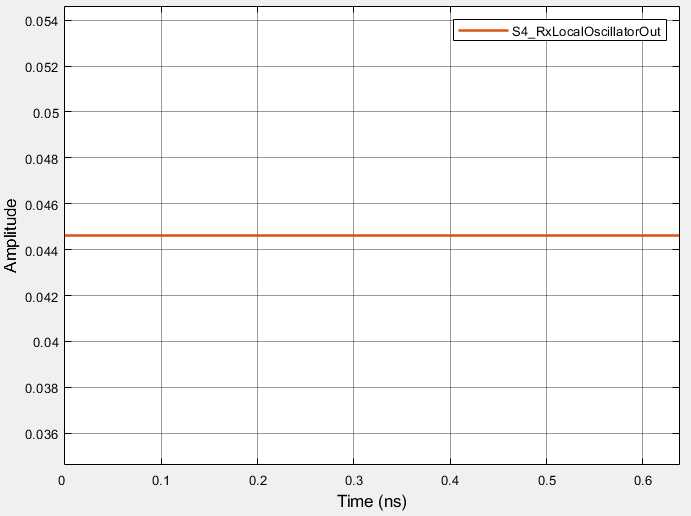
\includegraphics[scale=0.45]{./lib/local_oscillator/Figures/NoNoise.png}
    	\caption{Example of the generated signal with no noise }\label{Example_localOscillator}
\end{figure}

In the following examples the frequencyMismatch, laserRIN, laserLineWidth, opticalPower and phase are changed.
\begin{figure}[H]
	\centering
        \begin{subfigure}{.55\textwidth}
        \centering
        	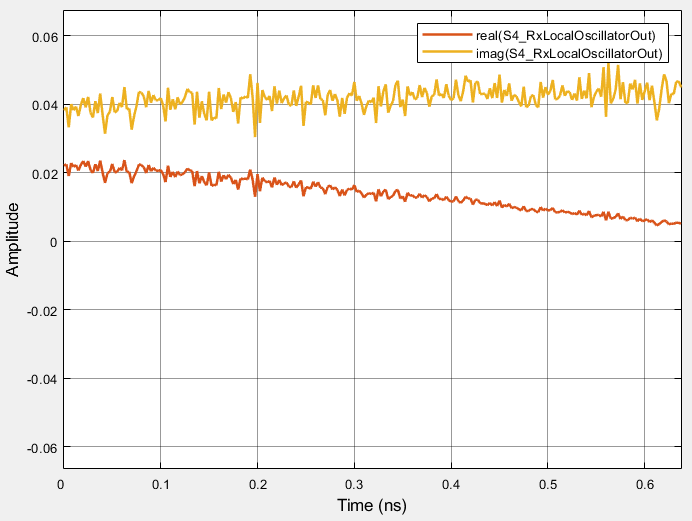
\includegraphics[scale=0.45]{./lib/local_oscillator/Figures/Tudo_100Mhz_10_pi_3_5e-14.png}
        \label{Example_All}\caption{Example of the generated signal with opticalPower=6dBm, phase=$\frac{pi}{3}$, laserRIN=5e$^{-14}$ and laserLineWidth=10Hz}
        \end{subfigure}%
        \begin{subfigure}{.55\textwidth}
        \centering
        	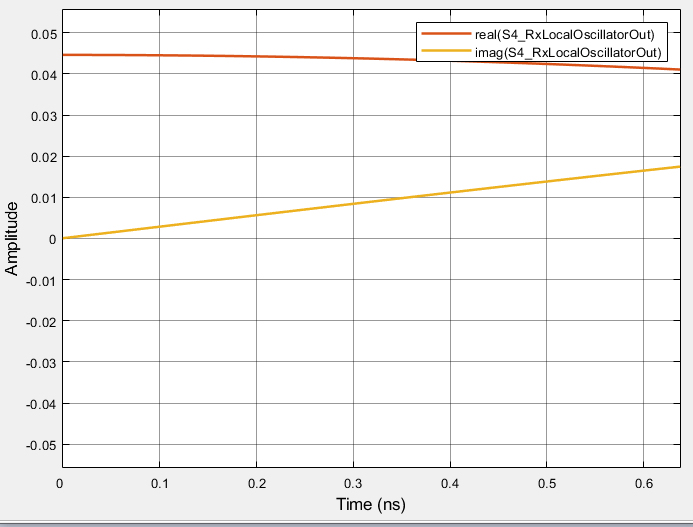
\includegraphics[scale=0.45]{./lib/local_oscillator/Figures/FrequencyMismatch_100MHz.png}
        	\caption{Example of the generated signal with frequencyMismatch=100MHz}\label{Example_FrequencyMismatch}
        \end{subfigure}
        \caption{}\label{Example_1}
\end{figure}

\begin{figure}[H]
	\centering
        \begin{subfigure}{.55\textwidth}
        \centering
        	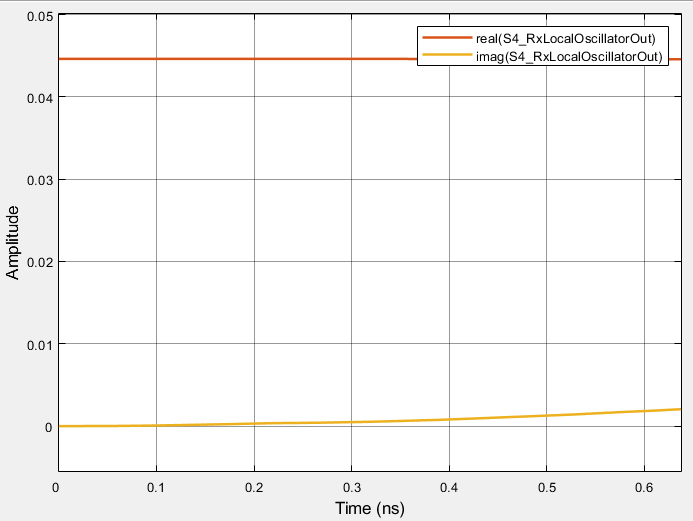
\includegraphics[scale=0.45]{./lib/local_oscillator/Figures/LineWidth_10.png}
        	\caption{Example of the generated signal \newline with laserLineWidth=10Hz }\label{Example_LineWidth}
        \end{subfigure}%
        \begin{subfigure}{.55\textwidth}
        \centering
        	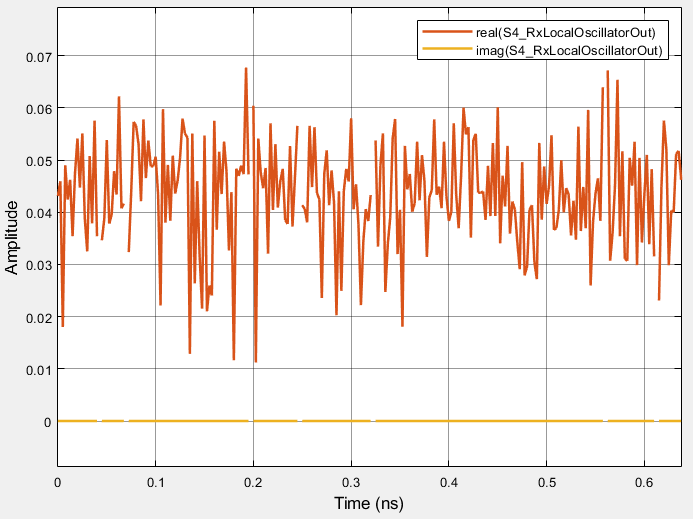
\includegraphics[scale=0.45]{./lib/local_oscillator/Figures/RIN_5e-13.png}
        	\caption{Example of the generated signal with laserRIN=5e$^{-13}$ }\label{Example_RIN}
        \end{subfigure}
        \caption{}\label{Example_2}
\end{figure}

\begin{figure}[H]
	\centering
        \begin{subfigure}{.55\textwidth}
        \centering
        	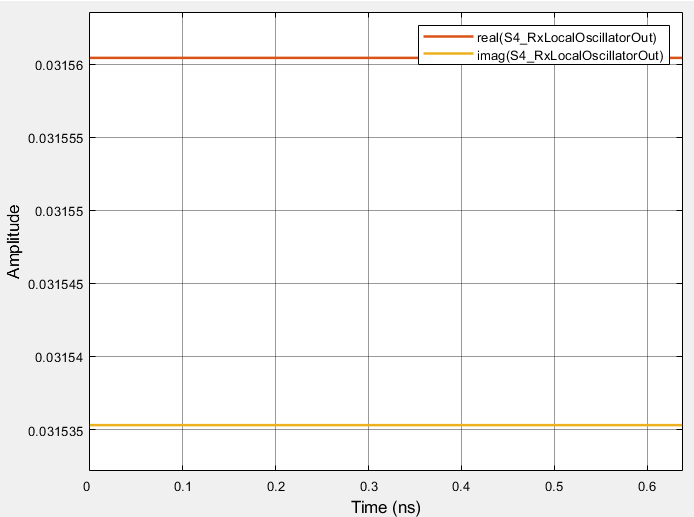
\includegraphics[scale=0.45]{./lib/local_oscillator/Figures/Phase_pi_4.png}
        	\caption{Example of the generated signal with phase=$\frac{pi}{4} $ }\label{Example_Phase}
        \end{subfigure}%
        \begin{subfigure}{.55\textwidth}
        \centering
        	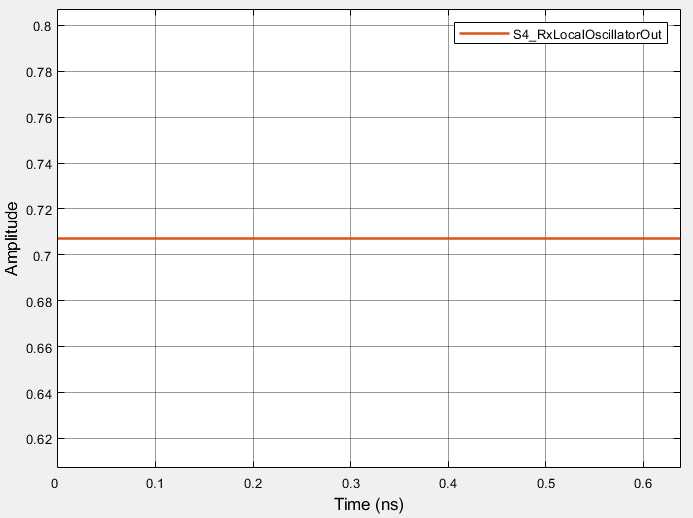
\includegraphics[scale=0.45]{./lib/local_oscillator/Figures/Power_30dBm.png}
        	\caption{Example of the generated signal with opticalPower=30dBm }\label{Example_Power}
        \end{subfigure}
        \caption{}\label{Example_3}
\end{figure}
The figures \ref{Example_1}, \ref{Example_2} and \ref{Example_3} shows that the phase was more affected by the frequencyMismatch and laserLineWidth, while the laserRIN affected more the amplitude.

\subsection*{Sugestions for future improvement}
A possible improvement would be the possibility to observe, in the frequency domain, the signals in the visualizer.

